\documentclass[border=7pt]{standalone}
\usepackage{tikz}
\usetikzlibrary{calc,patterns}
\begin{document}
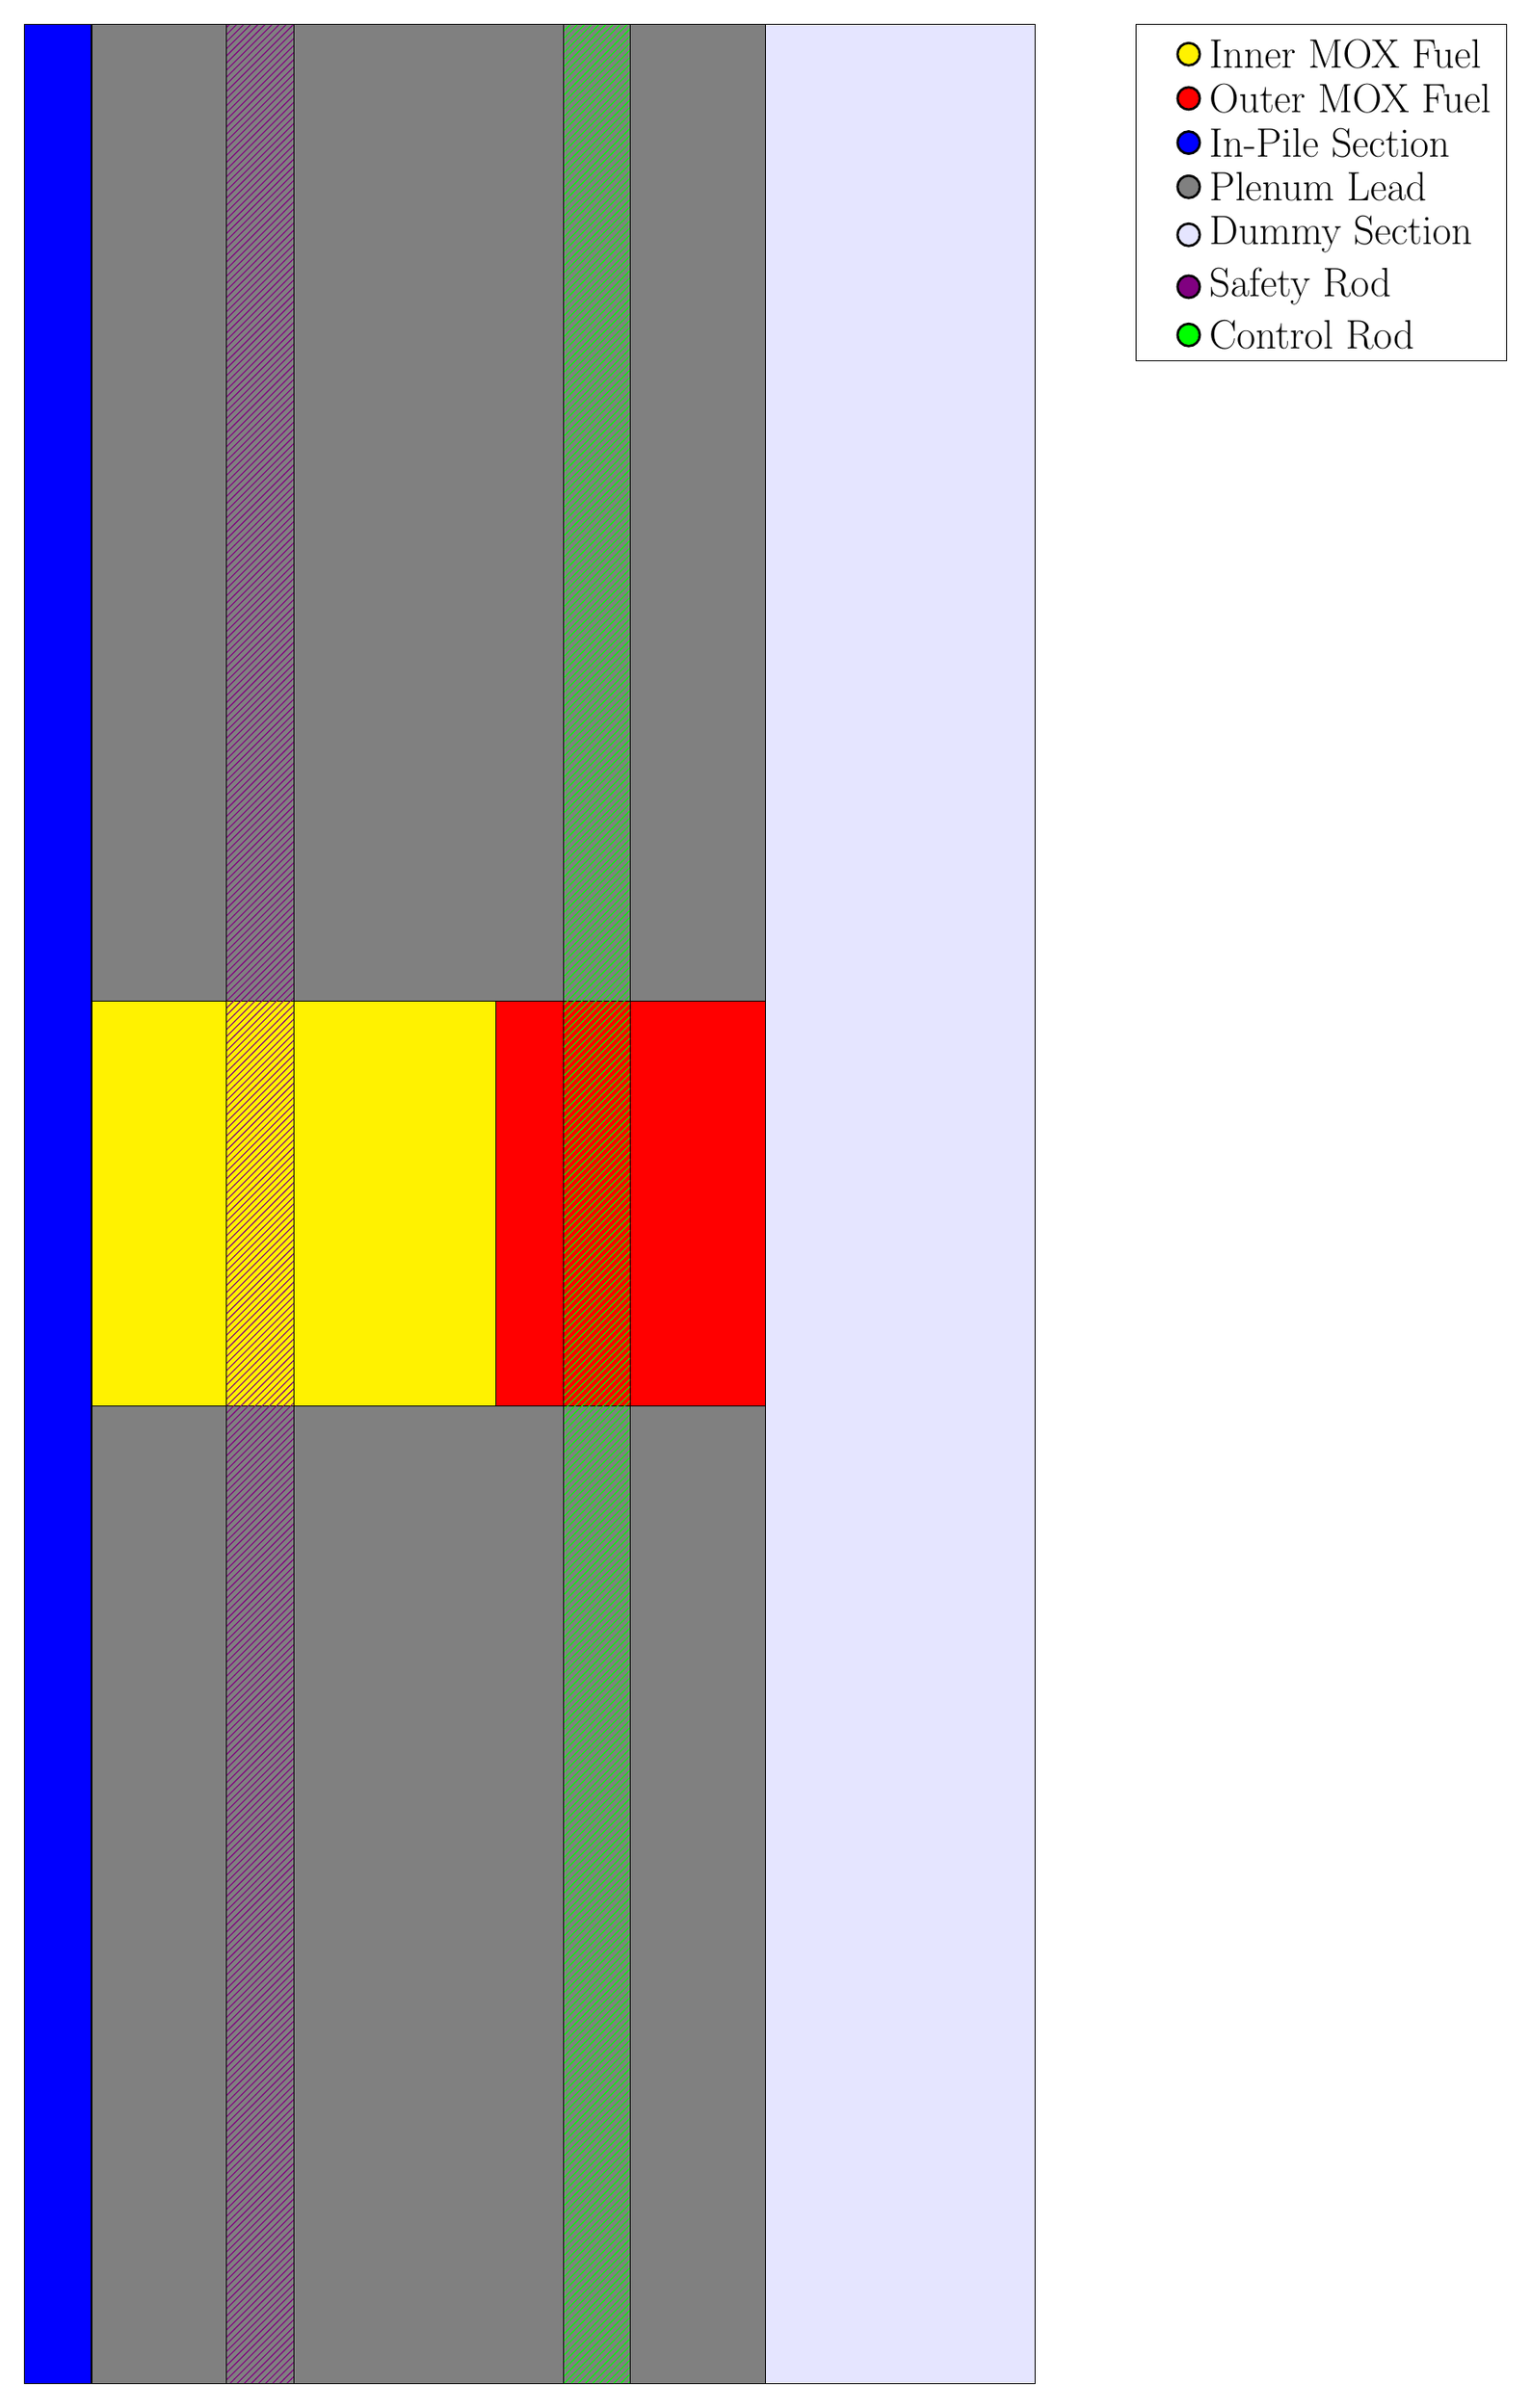
\begin{tikzpicture}[
  blacknode/.style={shape=circle, draw=black, line width=1, fill=gray },
  bluenode/.style={shape=circle, draw=black, line width=1, fill=blue },
  greennode/.style={shape=circle, draw=black, line width=1, fill=green },
  rednode/.style={shape=circle, draw=black, line width=1, fill=red },
  yellownode/.style={shape=circle, draw=black, line width=1, fill=yellow },
  violetnode/.style={shape=circle, draw=black, line width=1, fill=violet },   
  graynode/.style={shape=circle, draw=black, line width=1, fill=blue!10 },  
]

%PROFILE REACTOR
\filldraw[fill=blue!10, draw=black] (0,0) rectangle (15,35);

\filldraw[fill=blue, draw=black] (0,0) rectangle (1,35);
\filldraw[fill=gray, draw=black] (1,0) rectangle (11,14.5);
\filldraw[fill=yellow] (1,14.5) rectangle (7,20.5);
\filldraw[fill=gray, draw=black] (1,20.5) rectangle (11,35);
\filldraw[fill=red] (7,14.5) rectangle (11,20.5);
\draw[pattern=north east lines,pattern color=violet] (3,0) rectangle (4,35);

\draw[pattern=north east lines,pattern color=green] (8,0) rectangle (9,35);


%%LEGEND
\draw (16.5,30) rectangle (22,35);
\matrix [below left] at (current bounding box.north east) {
  \node [yellownode, label=right:\LARGE Inner MOX Fuel] {}; \\
  \node [rednode, label=right:\LARGE Outer MOX Fuel ] {}; \\
  \node [bluenode, label=right:\LARGE In-Pile Section] {}; \\
  \node [blacknode, label=right:\LARGE Plenum Lead] {}; \\
  
  \node [graynode, label=right:\LARGE Dummy Section] {}; \\
  
  \node [violetnode, label=right:\LARGE Safety Rod] {}; \\
  
  \node [greennode, label=right:\LARGE Control Rod] {}; \\
};


%\draw (0,0) -- (4,0);

%\shade[top color=yellow, bottom color=black] (0,0) rectangle (2,-1);
 %   \filldraw[fill=green!20!white, draw=green!40!black] (0,0) rectangle (2,1);
 %   \draw[pattern=north east lines,pattern color=red] (0,0) rectangle (1,3);
 %   \draw[pattern=north west lines,pattern color=blue] (0,0) rectangle (3,1);
%    \draw[pattern=vertical lines] (2,0) rectangle (5,1);
%    \draw[pattern=horizontal lines,pattern color=yellow] (2,0) rectangle (3,3);

\end{tikzpicture}
\end{document}